\chapter{Hawkeye Experimental Results}

\begin{figure}[htb]
\begin{center}
\ 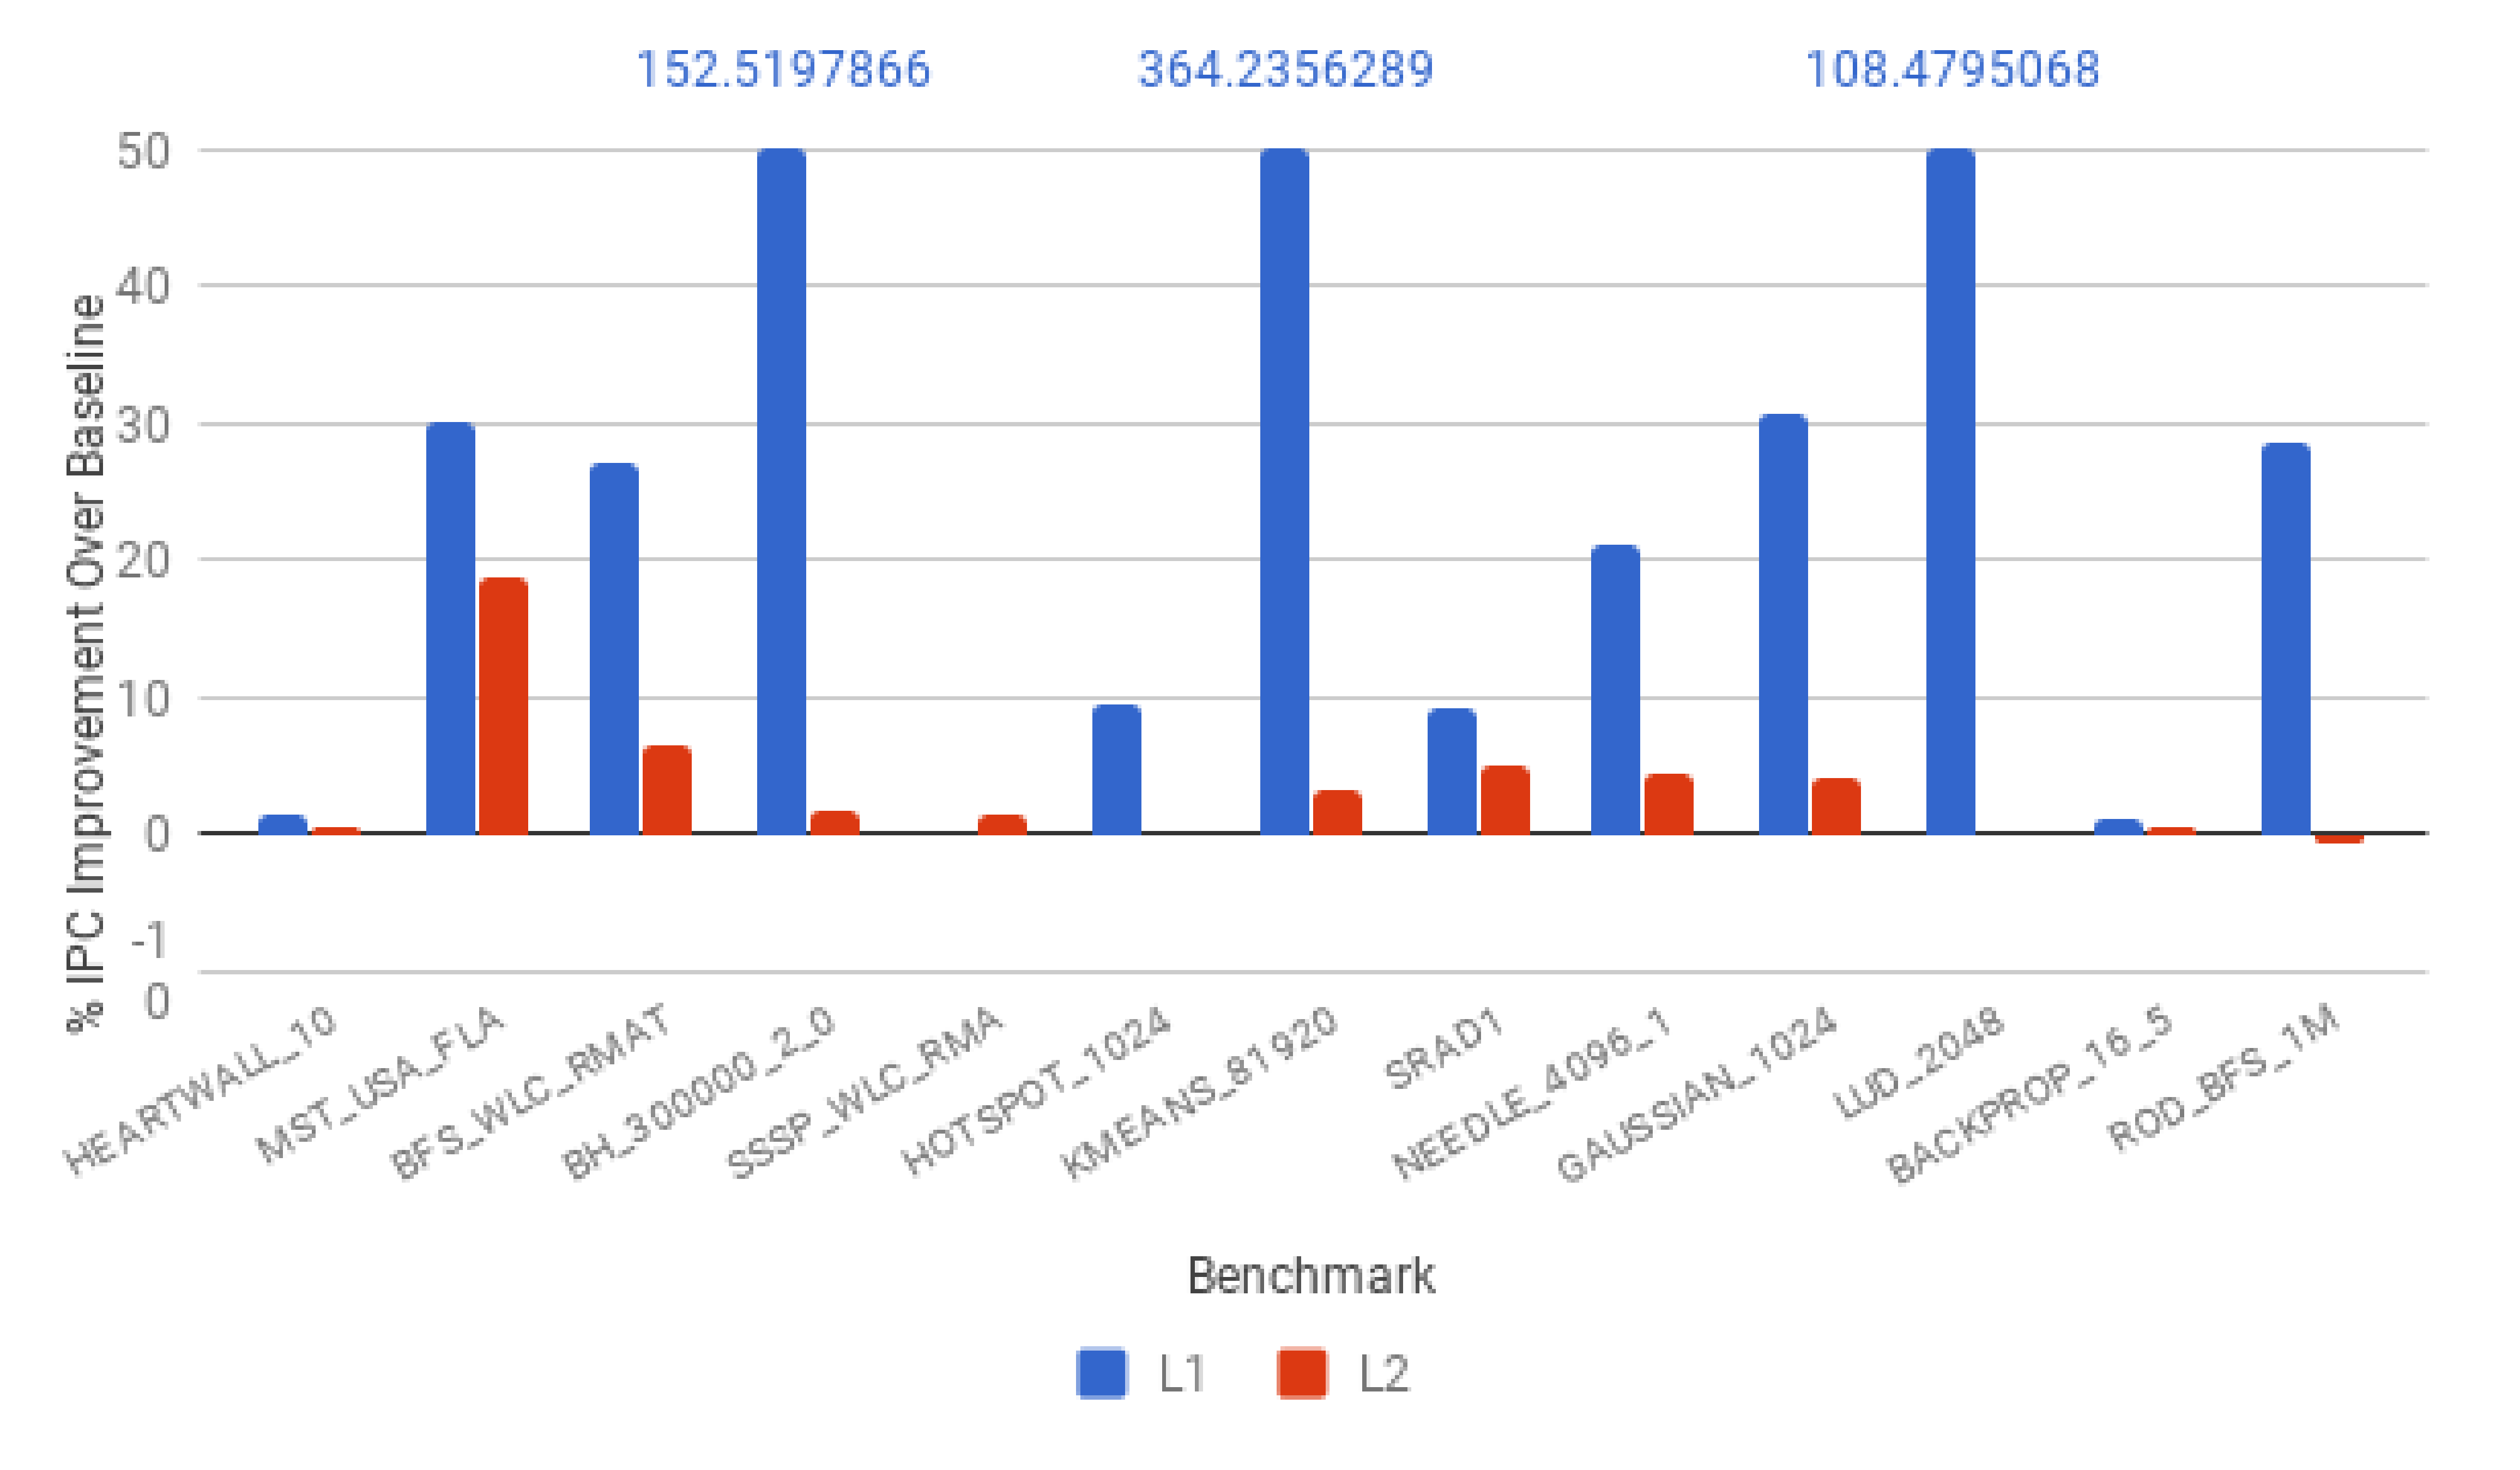
\psfig{file=figs/sensitivity.png,width=\textwidth}
\caption{Cache sensitivity for both L1 and L2 caches.} These numbers are percentage improvements over in IPC over baseline when quadrupling the size of each cache. Replacement for all cases is done with LRU.
\label{f:sensitivity}
\end{center}
\end{figure}

\begin{figure}[htb]
\begin{center}
\ \psfig{file=figs/l1_bias.png,width=\textwidth}
\caption{Average per-feature prediction bias for L1 caches. The bias denotes the percentage of truth values that agree with our predicted value of cache friendly or unfriendly. Here 50\% would be equivalent to a random prediction. The final column denotes our average per-feature bias across all benchmarks.}
\label{f:l1_bias}
\end{center}
\end{figure}

\begin{figure}[htb]
\begin{center}
\ \psfig{file=figs/l2_bias.png,width=\textwidth}
\caption{Average per-feature prediction bias for L2 caches.}
\label{f:l2_bias}
\end{center}
\end{figure}

\begin{figure}[htb]
\begin{center}
\ 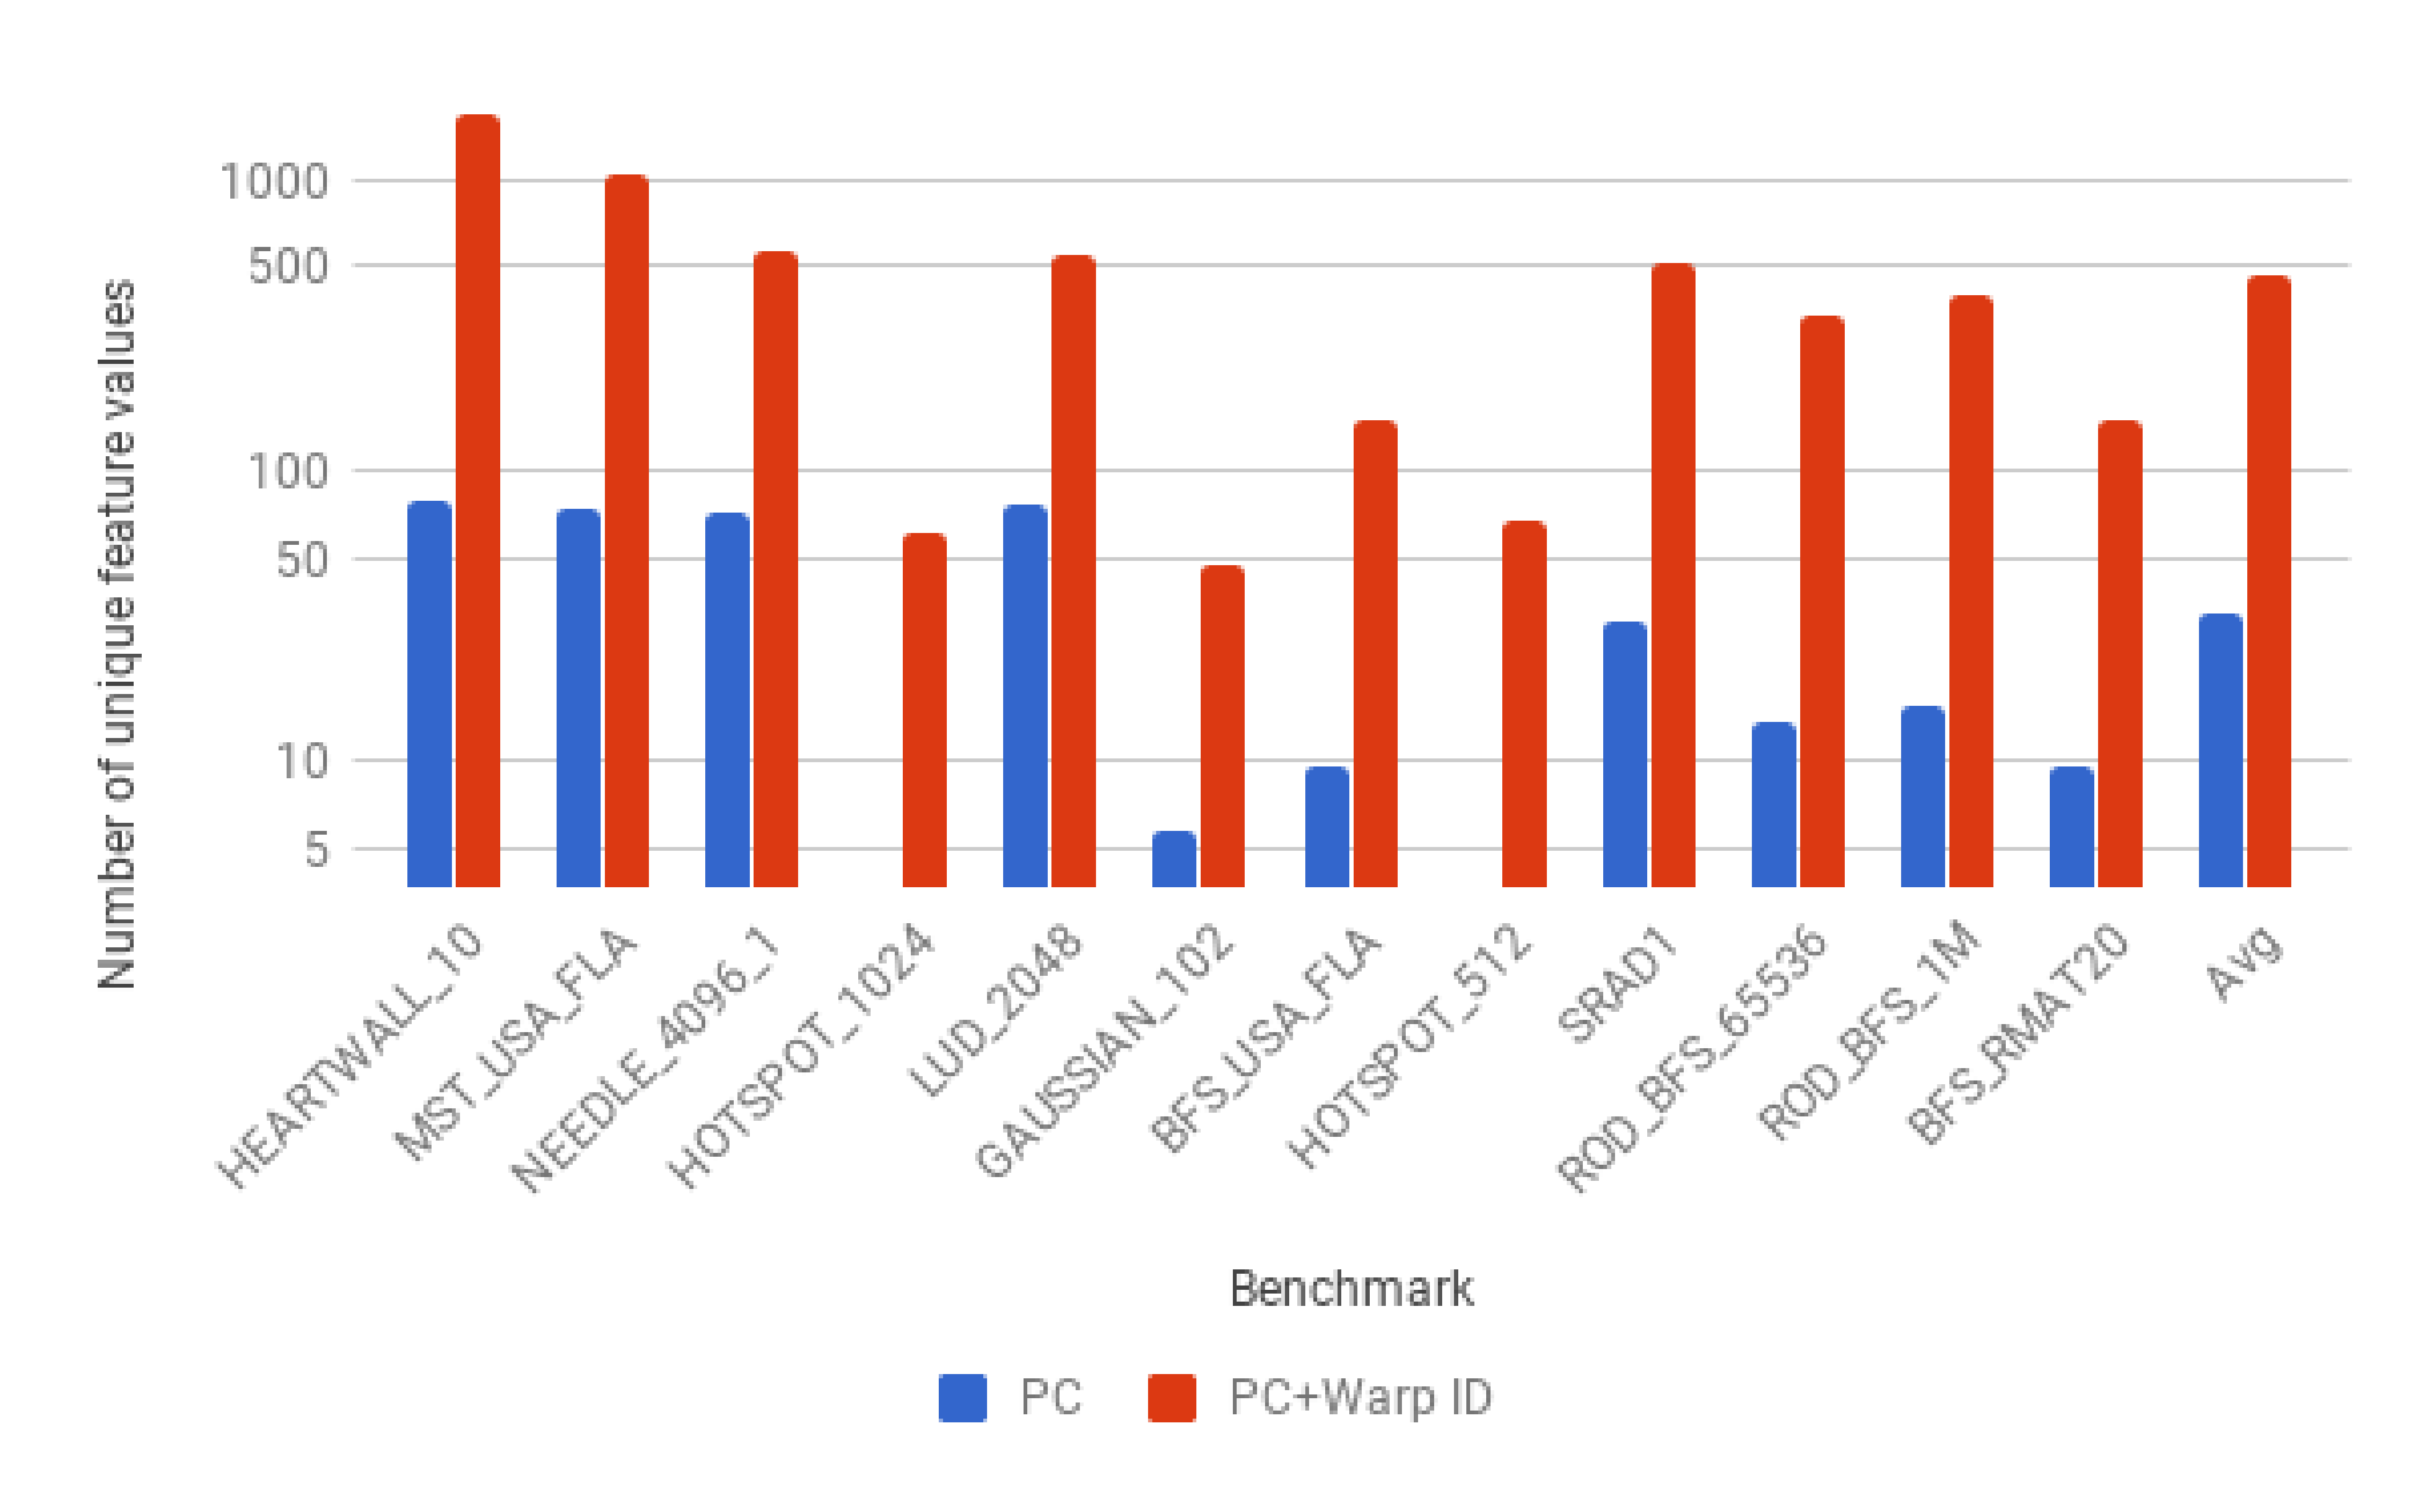
\psfig{file=figs/opt_uniq_vals.png,width=\textwidth}
\caption{Average unique values per feature at L1 and L2 caches.}
\label{f:opt_uniq_vals}
\end{center}
\end{figure}

\begin{figure}[htb]
\begin{center}
\ 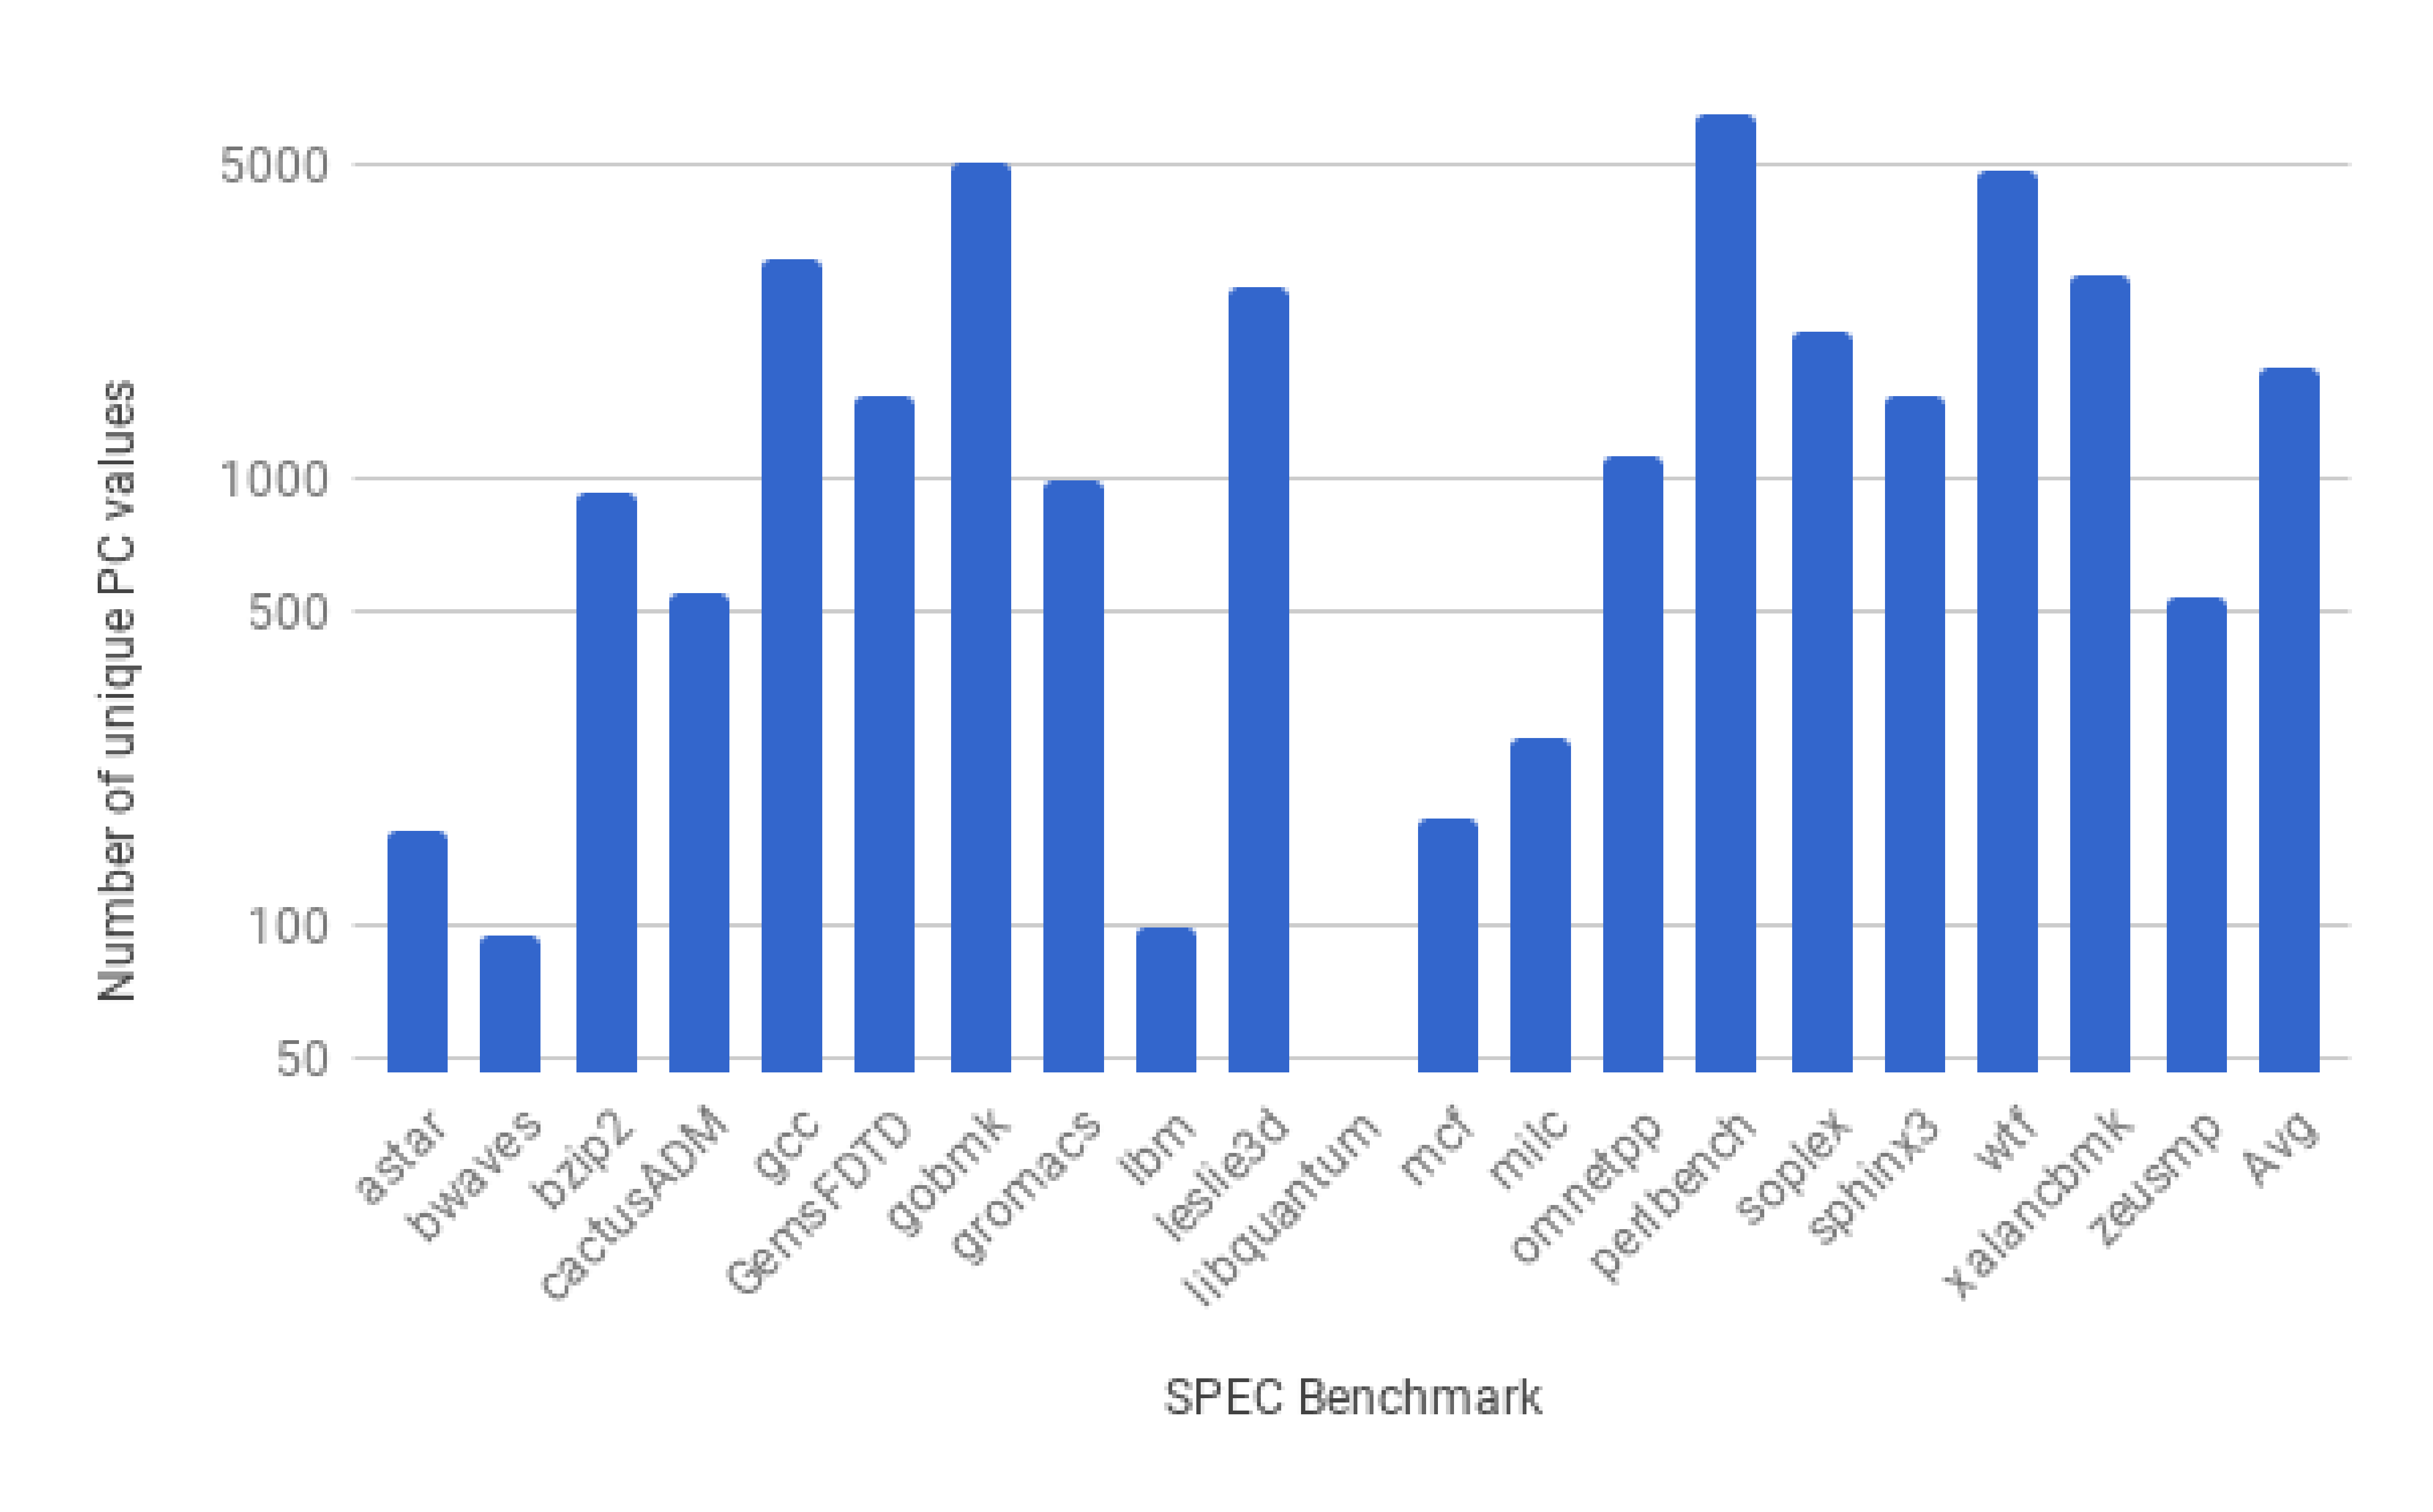
\psfig{file=figs/cpu_opt_uniq_vals.png,width=\textwidth}
\caption{Number of unique PC values seen on CPU SPEC Benchmarks. Notice that these numbers are roughly on the same order of magnitude as the number of PC+WID hashed values we see on GPU.}
\label{f:cpu_opt_uniq_vals}
\end{center}
\end{figure}

\begin{figure}[htb]
\begin{center}
\ \psfig{file=figs/l1_miss_rate.png,width=\textwidth}
\caption{Average miss rate improvement over LRU for L1 caches. This improvement is measured in percentage points over the miss rate observed with LRU.}
\label{f:l1_miss_rate}
\end{center}
\end{figure}

\begin{figure}[htb]
\begin{center}
\ \psfig{file=figs/l2_miss_rate.png,width=\textwidth}
\caption{Average miss rate improvement over LRU for L2 caches. This improvement is measured in percentage points over the miss rate observed with LRU.}
\label{f:l2_miss_rate}
\end{center}
\end{figure}
